\documentclass[11pt,a4paper]{report}
\usepackage[hmargin=3cm,vmargin=3cm]{geometry}
\usepackage{graphicx}
\usepackage{caption}
\usepackage{array}
\usepackage{listings}
\graphicspath{Images}
\usepackage{xcolor}
\usepackage[section]{placeins}
\usepackage[final]{pdfpages}
\usepackage[urlcolor  = blue,
 	colorlinks=true,
    allcolors = blue,	`1Q
    linktocpage=true,]{hyperref}
\usepackage{color}
\usepackage[cache=false]{minted}
\usepackage{filecontents}
\usepackage[comma,sort,round]{natbib}
\usepackage{url}
\usepackage[toc,page]{appendix}
\usepackage{verbatim}
\renewcommand{\bibname}{References} 

\begin{document}
\begin{figure}
\centering

\includegraphics[width = 0.3\textwidth]{iit}
\hspace{1cm}

\includegraphics[width = 0.4\textwidth]{fossee-logo.png}
\end{figure}

\title{\textbf{\textbf{Osdag Documentation}}\vspace{20mm} \\
\small Under the guidance of \\ \vspace{5mm}
\large \textbf{Prof.Siddhartha Ghosh} \vspace{1mm}\\ Civil Engineering Department \\ IIT Bombay \\
}

\title{\textbf{\textbf{Osdag Documentation}}}

\newpage
\maketitle



\tableofcontents

\chapter{\textbf{Introduction}}

\section{What is Osdag?}

\noindent Osdag is Free/Libre and Open Source Software being developed for design of steel structures. Its source code is written in Python, 3D CAD images are developed using PythonOCC. Github is used to ensure smooth workflow between different modules and team members. It is in a path where people from around the world would be able to contribute to its development. FOSSEE's ``Share alike'' policy would improve the standard of the software when the source code is further modified based on the industrial and educational needs across the country.

\noindent Osdag is created both for educational purpose and industry professionals. As Osdag is currently funded by MHRD, Osdag team is developing software in such a way that it can be used by the students during their academics and to give them a better insight look in the subject.

\noindent Osdag can be used by anyone starting from novice to professionals. It's simple user interface makes it flexible and attractive than other software. Video tutorials are available to help get started. The video tutorials of Osdag can be accessed \href{https://osdag.fossee.in/resources/videos}{here}.

\section{Who is this documentation for?}

\noindent One of the main aim of Osdag is that any civil/structural engineer or practicing professional to be able to contribute to development of this software. If any professional/Company feels that design a certain member/connection or addition of certain cross section would help them they can make changes to the source code to cater their requirements. They can send pull request on our github accounts and if the additions are found within the guidelines and correct we will publish the changes/additions.

This documnetation will guide on how to incorporate your "piece of code" into this software. It also lays out the guidelines one must follow to modify the code.

\section{Structure of This Documentation}

\noindent First Chapter details on the class hierarchy followed. Second chapter details on how to modify the UI. There are three UIs in this software. One for mainpage one is module window and one is design preference tab. One can modify all these with simple commands in their module without having to touch the UI file. Third chapter is how to edit the design report. Fourth chapter is algorithms followed by each module. Fifth one is about dependencies, How to make the installer or modify the installer. DDCL of all modules are attached as Appendices.


\chapter{\textbf{Class Hierarchy}}
\section{Hierarchy of Modules}
\noindent Figure below chows the classes, hierarchy and folder structure.
\begin{center}
	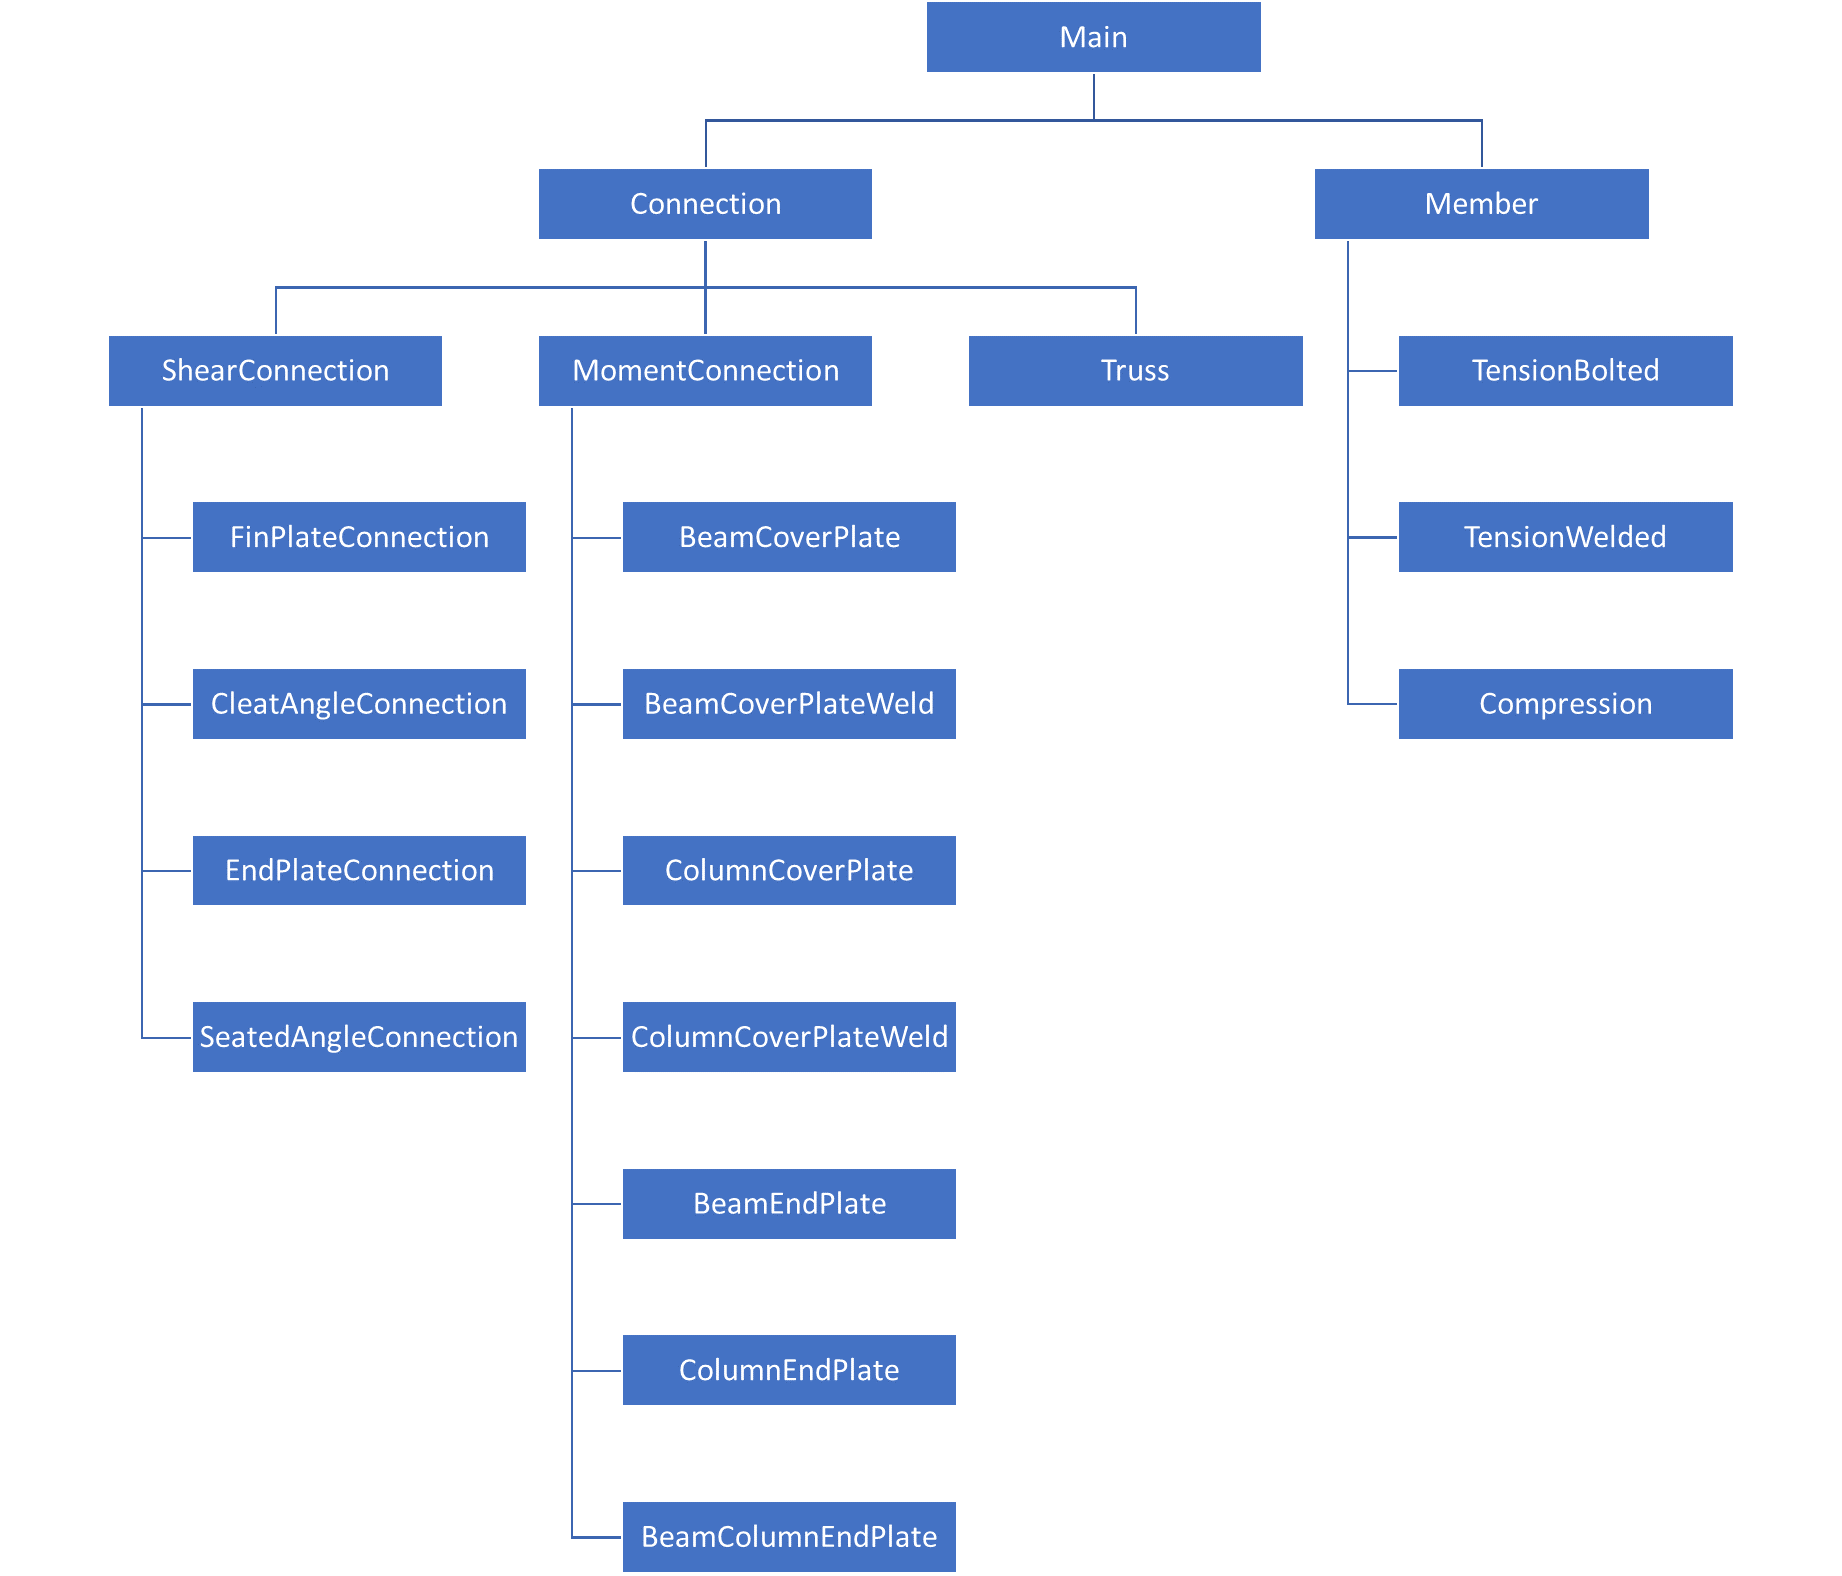
\includegraphics [width=15cm]{Class_Hierarchy.png}
\end{center}

\section{Hierarchy of Components}
\noindent *** Is This Required ***

\section{Hierarchy of CAD}
\noindent **** Is This REquired? ***

\chapter{\textbf{Creating UI}}
\section{Additing New Module}
\noindent ****** Under Progress ***.\\
\noindent Easier way to add new module without having to use qt designer or UI file is under development. May be there should be a button "Add New Module" In Which User gives where the new module is under Hierarchy, name of the module, image of the module (for radio button) and it should create a .py file in corresponding folder based on Hierarchy with appropriate file name and add This classname (class name shall be fixed. It can be whatever name your gives for Module, Spaces removed). This class Shall have all mandatory functions.

\section{Creating/Modifying Input Dock in Module}
\noindent Input dock contains lable and input field. To generate each field, developer shall specify five inputs in the following format.
[KEY, Lable Name, Type of Input Field, Existing Values in Input Field, Default Values]

KEY is the Key of the input dictionary.This is also the 'object name' of input box you are creating.\\ 
Lable name is the name displayed to the left of input field
Type of input field can be one of the following:
\begin{itemize}
\item textbox (TYPE\_TEXTBOX)
\item drop down (TYPE\_COMBOBOX)
\item Tile (TYPE\_TITLE)
\item Image (TYPE\_IMAGE)
\item Module Name (TYPE\_MODULE)
\item customized popup (TYPE\_COMBOBOX\_CUSTOMIZED)
\end{itemize} 

Default values is the initial values you want to display input field. This is ususally kept empty('None') for text box. For combobox, the initial list you want to display should be passed here.

Example:

Creating input dock for gusset plate.




\section{Creating/Modifying Output Dock in Module}
\noindent For Beam Column End plate design I have added python code for weld design between beam and end plate. Concerned code is attached vide \hyperlink {page.102}{Appendix-G}.

\section{Settingup log file}
\noindent Log file setup can be done by just adding this python function \hyperlink {page.10}{Appendix-A} in your module file. The function generates log messages for log file 'logging\_text.log', for run terminal and for textarea in module\_window ui. Log messages can be generated using logger.info(error message), logger.warning(error message) and logger.error(error message). To change the color of warning, error or information messages in UI, just edit the color in span style in the function handle() of class OurLog.

\section{Generating Warning/Error message box}
\noindent QMessageBox can be used to generate messagebox for error messages in ui. Concerned code is attached vide \hyperlink {page.12}{Appendix-B}.

\section{Design\_Preferences UI}
\noindent Design\_preference UI contains multiple tabs based on items of tab\_list() function in module file. Each tab is specified by a tuple with three elements.. tab\_name, tab\_type(There are two types: One with buttons to update database and one without buttons) and function\_name(Which contains all the items to be shown in the tab - it is similar to input\_values() function of input dock). Concerned code is attached vide \hyperlink {page.13}{Appendix-C}.

\nocite{*}
\newpage
\bibliographystyle{unsrtnat}
\bibliography{references}

\begin{appendices}
	\chapter{Log File Setup}
	\inputminted[%
	breaklines,
	mathescape,
	firstline=190,
	lastline=216,
	linenos,
	numbersep=5pt,
	frame=single,
	framesep=5pt,
	numbersep=5pt,
	fontsize=\small,
	]{python}{../Osdag3-master/gusset_connection.py}
	\inputminted[%
	breaklines,
	mathescape,
	firstline=167,
	lastline=184,
	linenos,
	numbersep=5pt,
	frame=single,
	framesep=5pt,
	numbersep=5pt,
	fontsize=\small,
	]{python}{../Osdag3-master/gusset_connection.py}
	\chapter{Warning/Error message box}
	\inputminted[%
	breaklines,
	mathescape,
	firstline=126,
	lastline=130,
	linenos,
	numbersep=5pt,
	frame=single,
	framesep=5pt,
	numbersep=5pt,
	fontsize=\small,
	]{python}{../Osdag3-master/gusset_connection.py}
	\chapter{Design\_preference UI}
	\inputminted[%
	breaklines,
	mathescape,
	firstline=324,
	lastline=366,
	linenos,
	numbersep=5pt,
	frame=single,
	framesep=5pt,
	numbersep=5pt,
	fontsize=\small,
	]{python}{../Osdag3-master/gusset_connection.py}
\end{appendices}
\begin{comment}
\begin{appendices}
	\addtocontents{toc}{\protect\setcounter{tocdepth}{0}}
	\chapter{DDCL for Fin plate}
	\includepdf[pages=-]{../FinPlate/FinPlate.pdf}

	\chapter{DDCL for Cleat angle}
	\includepdf[pages=-]{../CleatAngle/CleatAngle.pdf}

	\chapter{DDCL for End plate}
	\includepdf[pages=-]{../FlexibleEndPlate/FlexibleEndPlate.pdf}

	\chapter{Fin Plate design caluclations using python}
	\inputminted[%
	breaklines,
	mathescape,
	firstline=241,
	lastline=405,
	linenos,
	numbersep=5pt,
	frame=single,
	framesep=5pt,
	numbersep=5pt,
	fontsize=\small,
	]{python}{../pythoncodes/finPlateCalc.py}

	\chapter{Imported file get\_bolt\_values}
	\inputminted[%
	breaklines,
	mathescape,
	linenos,
	numbersep=5pt,
	frame=single,
	framesep=10pt,
	numbersep=5pt,
	fontsize=\small,
	]{python}{../pythoncodes/get_bolt_values.py}
	
	\chapter{Imported file get\_weld\_values}
	\inputminted[%
	breaklines,
	mathescape,
	linenos,
	numbersep=5pt,
	frame=single,
	framesep=10pt,
	numbersep=5pt,
	fontsize=\small,
	]{python}{../pythoncodes/get_weld_values.py}

	\chapter{Stiffener design in Beam Column End Plate using Python}
	\inputminted[%
	breaklines,
	mathescape,
	linenos,
	firstline=788,
	lastline=858,
	numbersep=5pt,
	frame=single,
	framesep=10pt,
	numbersep=5pt,
	fontsize=\small,
	]{python}{../pythoncodes/bc_endplate_calc.py}
\end{appendices}
\end{comment}

\end{document}



